%# -*- coding: utf-8-unix -*-

%\bibliographystyle{sjtu2}%[此处用于每章都生产参考文献]
\chapter{绪论}
\label{chap:intro}

运行Android系统的设备数量随着移动互联网的兴起爆发式增长,2014年著名的视频网站YouTube超过一半的流量来自于移动设备[1]。

根据Google公司的统计,截止2015年9月30日,在全球范围内已激活的Android设备已经达到14亿台[2],超过微软公司的Windows,苹果公司的Mac OS和iOS,是全球运行设备数量最多的商用操作系统。

\section{Android生态系统}
\label{sec:android_ecosystem}

通常每台智能手机运行着数十至上百个应用程序,简称App。
其中一部分是制造设备的厂商或定制Android操作系统厂商的App,但用户每天接触时间最长的是第三方的应用厂商或者独立开发者开发的,并且需要连接互联网的App。

在Android生态系统中,开发者完成Android App的开发完后,需要通过诸如Google Play Store、腾讯应用宝、小米应用商店等Android应用市场发布App,应用市场会对开发者提交的App进行安全、内容和程序稳定性上的审核,通过审核后,用户再从应用市场搜索App进行下载安装和使用,流程如图\ref{fig:IndustryChain}所示。
%TODO 引用艾媒咨询

\begin{figure}[!htp]
	\centering
	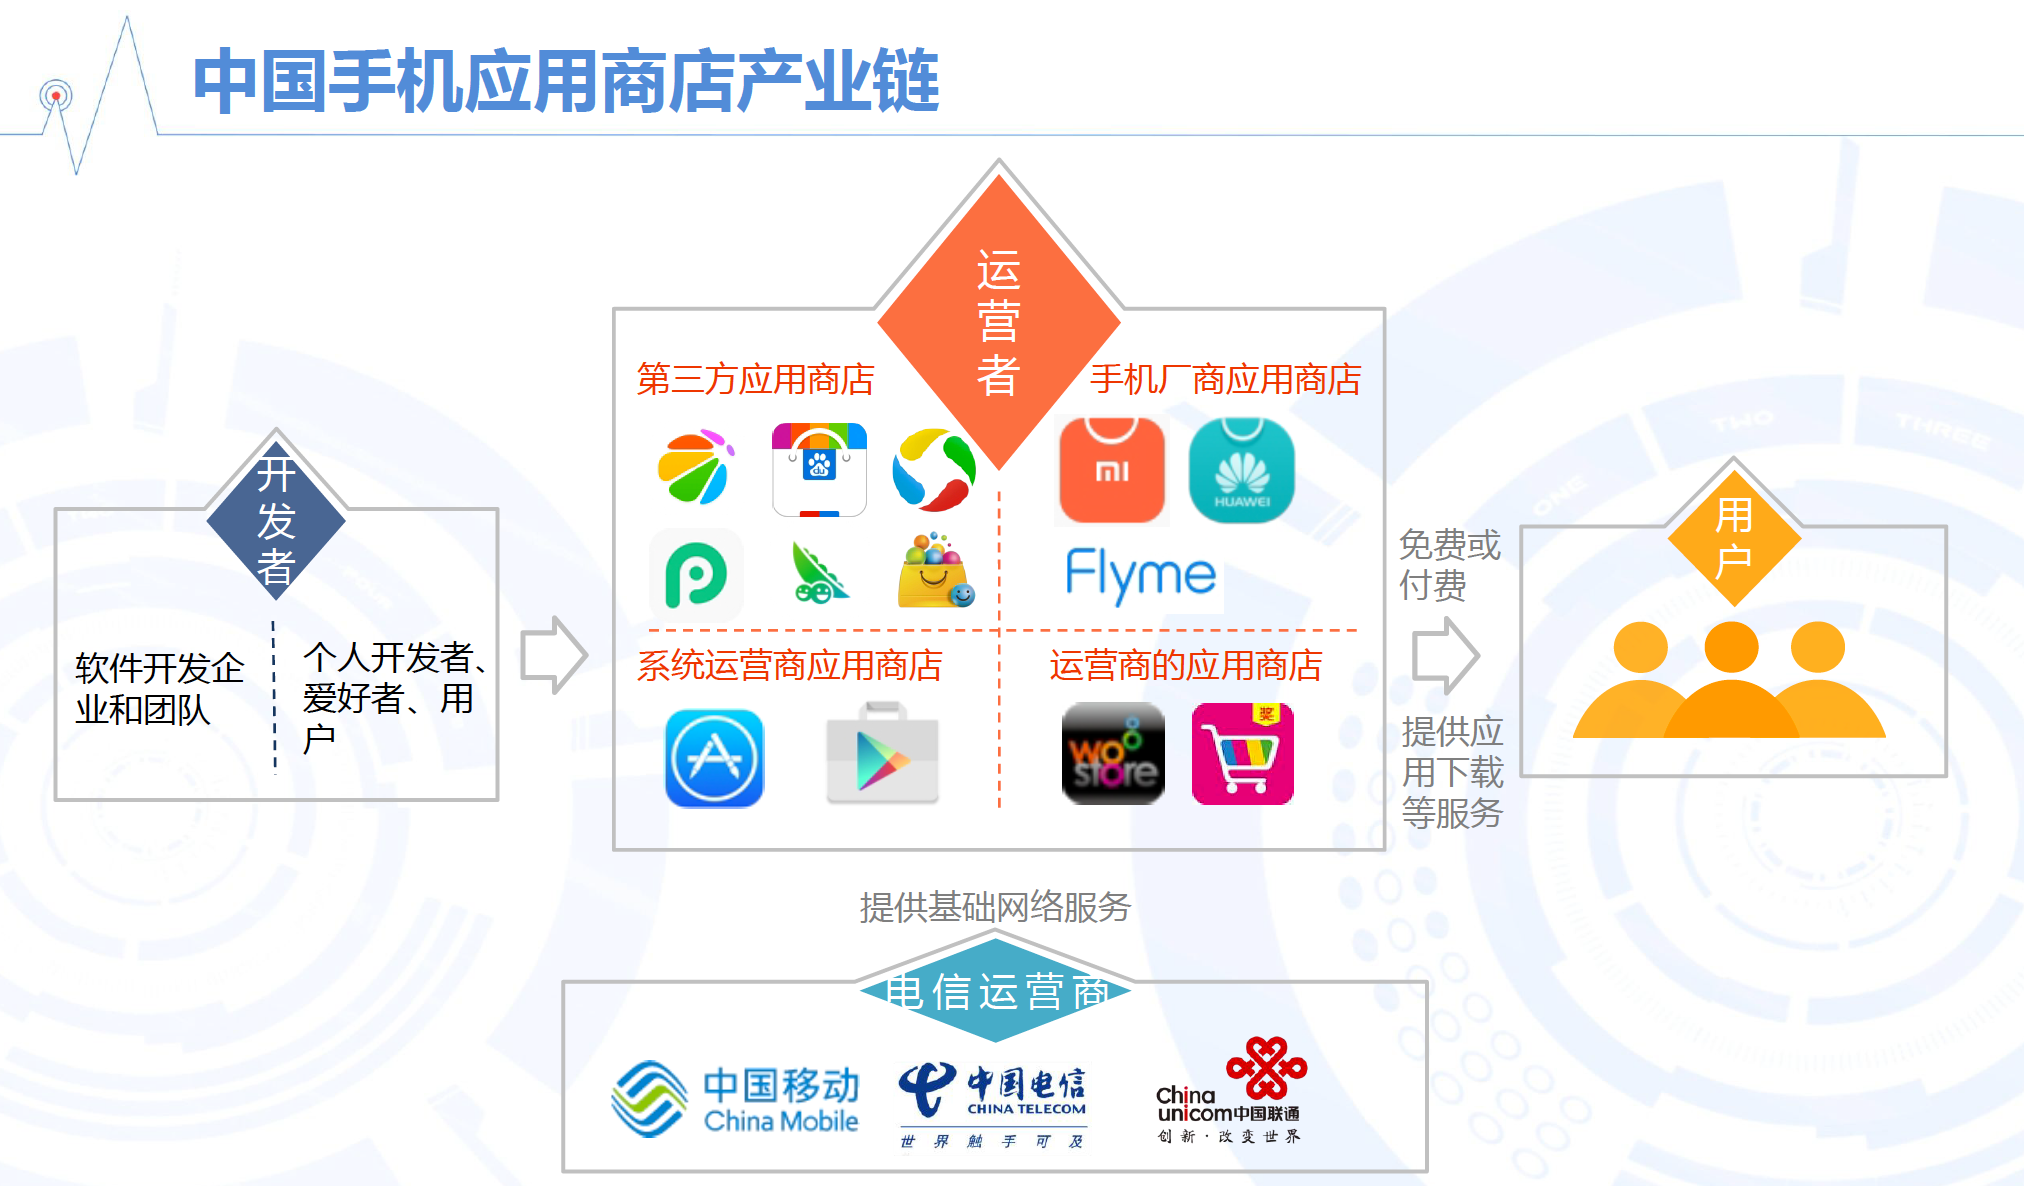
\includegraphics[width=1\textwidth]{industry_chain.png}
	\bicaption[fig:IndustryChain]{这里将出现在插图索引中}{中国手机应用商店产业链}{Fig}{Mobile App store industry chain in China}
\end{figure}

\subsection{用户信息价值}

从用户处获得信息反馈,根据反馈信息改进App的设计与体验、调整运营方式是移动互联网生态链中很重要的一个环节,因为用户体验直接影响到App的用户数量。

部分用户反馈可以通过应用市场的打分和评价中体现,但这些反馈包含的信息太少,只有简单的文字描述和分数评价,只能对其他用户起参考作用,难以进行更加深入的分析获取有价值的数据,对开发团队价值较小。除此之外,从应用市场得到的App反馈信息受制于应用商店,还会存在恶意竞争和刷单等问题,是App开发运营团队不可控的。

\subsection{碎片化}

Android操作系统的一大问题是碎片化[3],全球各个手机厂商都有不计其数的不同型号的手机运行着不同版本的Android操作系统,这些手机的硬件参数不同,系统版本不一。但有“开放手机联盟(Open Handset Alliance)”的存在,规定了生产运行Android系统的设备都需要满足一定的兼容性要求,这使得Android App能够运行在绝大部分遵守规范的Android设备上,一定程度上增强了这个松散阵营的兼容性。

Android碎片化主要包括设备碎片化和系统版本碎片化。
设备碎片化是指不同厂商不同型号的设备,在硬件配置上的不同。
例如Android手机使用各种各样的屏幕,这些屏幕的参数包括尺寸、分辨率、电容屏或电阻屏、是否支持压力、多点触控支持的上限等,不同的屏幕参数对于App的使用体验不一样,尤其是分辨率,直接涉及到App前端显示的内容多少。
除了屏幕以外,CPU、GPU、内存、摄像头等硬件的参数同样多种多样,造成的影响就是在不同型号的Android设备上运行同一个App,产生的效果截然不同。

系统版本碎片化是指不同的设备运行了不同版本的Android系统,不同版本系统号提供的API和库实现不一样,变动较大的版本号之间系统底层的机制也会不一样,每个Android App都指定了能够运行的系统大版本号范围。
Android系统版本非常复杂,当前情况下由Google公司主导“Android Open Source Project”,简称AOSP,该分支开放给开源社区,属于最纯净的Android分支,通常意义上的Android系统大版本号跟随的是AOSP分支。
Google公司的Nexus系列设备,运行的是Google公司融合了AOSP和不开源的Google Framework的ROM,通常被称为原生Android ROM。
但在中国,用户使用更为广泛的是各大厂商基于AOSP修改定制的Android操作系统,以小米公司的MIUI为代表。绝大部分能在AOSP上运行的App同样能够运行在这些系统上,但这些系统在一些地方对AOSP源码做了修改,行为会稍有不同,这些不同点容易产生意想不到的问题。

截止2016年5月23日,距离Android 6.0版本发布近一年,该版本的市场占有率还不足10\%,如图\ref{fig:androidVersion}所示是当前Android版本分布。
%TODO引用http://www.appbrain.com/stats/top-android-sdk-versions

\begin{figure}[!htp]
	\centering
	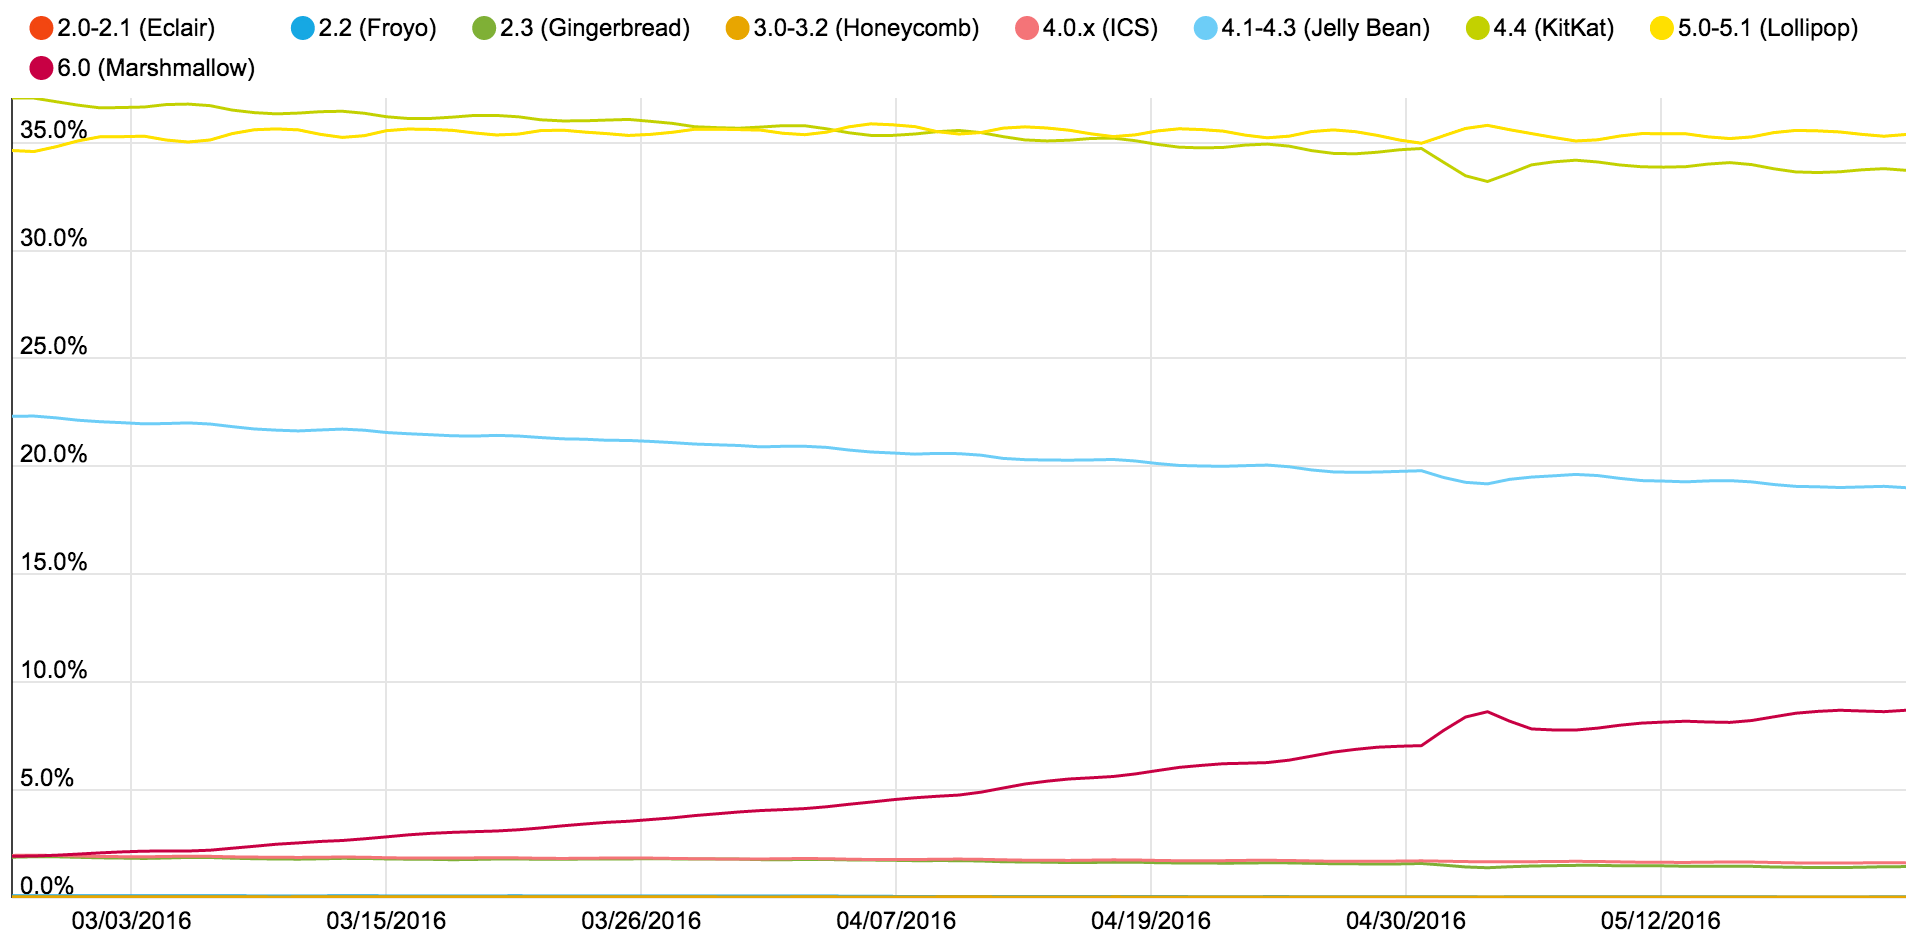
\includegraphics[width=1\textwidth]{android_version.png}
	\bicaption[fig:androidVersion]{这里将出现在插图索引中}{Android系统版本分布}{Fig}{Android system version distribution}
\end{figure}

\subsection{存在的问题}
\label{subsec:exist_problem}

对于软件开发者,实现从所有用户设备中收集App的使用状况,需要考虑大规模并发、持久化存储、稳定性等各种问题,难度高而且工作量大。对于大团队或许有能力实现收集反馈信息的功能,但对于想要了解用户使用状况的独立开发者,开发这类功能的工作量过大,甚至会超过了App业务功能本身。

除此之外,开发者还要面对硬件参数各异、运行各种版本系统的用户设备,保证开发的App在碎片化的Android设备上不崩溃,并且都拥有较为良好的用户体验。开发团队在测试阶段不可能覆盖所有的Android设备,并且测试也难以覆盖所有情况。
存在一种情况,在绝大部分设备上都能正确运行的App,在某款用户量很少的Android设备上会崩溃,导致这部分用户无法正常使用。
如果能够将这款设备的App崩溃信息发送给开发者,开发者就能够定位并解决问题,通过更新App提高兼容性和稳定性。

\section{项目解决的问题}
\label{sec:solve_problem}

本文介绍的工具代号“Appetizer”,解决的是\ref{subsec:exist_problem}小节中描述的问题。“Appetizer”包括一个能够集成在Android应用中的轻量级软件开发工具包,简称为客户端SDK,和具有良好可扩展性的用于接收并处理数据的服务端程序。

Appetizer客户端SDK能够收集用户使用App的操作路径和时间,在App崩溃时收集程序调用栈和设备相关状态信息,侦测Android应用程序未响应事件,记录App每次启动时的黑白屏时间,存储这些使用信息,并在网络条件允许的情况下将收集到的信息发送到服务端。

Appetizer服务端能够持久化存储客户端SDK发送的消息,对App使用信息做处理和统计分析,展现有价值的内容给App的开发团队和运营团队,包括日活跃用户、崩溃信息分类、机型统计等处理过的数据。

Appetizer客户端SDK的特点是轻量和稳定。不使用任何第三方库,尽可能减小SDK的空间占用,减少使用该SDK的App的空间占用增加。同时保证稳定性,不会因为SDK本身的问题造成App崩溃。Appetizer服务端在架构上保证了良好的可扩展性,可以通过简单的增加服务器数量承受更大的流量压力。

\section{相关工具产品}
\label{sec:related_work}

中国市场上,提供用户行为分析统计和崩溃信息收集的商业产品主要有腾讯Bugly,友盟[4]和TalkingData[5]。他们的产品对于Android App用户行为分析方面的功能包括用户活跃度、用户构成、渠道分析、页面访问路径统计、事件转化率等,主要是对session统计得到的数据进行处理的结果,其中腾讯Bugly对应用崩溃信息分析处理功能较强。

国际市场上,提供相关功能的商业产品主要有Google FireBase,Yahoo Flurry Analytics[6]和Twitter Fabric。其中Google FireBase同时包括用户行为统计和崩溃信息收集,其他功能也较为丰富,是Google公司主推的Android开发者服务工具。Flurry Analytics可以对用户行为统计数据进行较为复杂的分析和报表输出。Fabric可以将所有用户的App崩溃信息反馈给开发团队,并且还有一整套团队测试工具进行辅助。

开源软件ACRA[9]是做Android App崩溃信息统计的工具,因为是开源软件需要使用者自己搭建服务端,崩溃信息收集功能完善并且发送的信息有很好的可定制性。

国内外的学术界也有对Android应用的用户使用行为进行分析的研究[7][8]。

\section{本章小结}

本章是整篇文章的绪论,描述了整篇文章研究的主要问题。

\ref{sec:android_ecosystem}节介绍了Android生态系统的大致流程、碎片化的问题和整个生态系统面临的问题,\ref{sec:solve_problem}节介绍了“Appetizer”的主要功能、特点和能够解决的问题,\ref{sec:related_work}节列出了国内外解决Android生态问题的相关商业产品和开源产品以及它们的特点。
